% Created 2019-07-10 Mi 03:35
% Intended LaTeX compiler: pdflatex
\documentclass[11pt]{article}
\usepackage[utf8]{inputenc}
\usepackage[T1]{fontenc}
\usepackage{graphicx}
\usepackage{grffile}
\usepackage{longtable}
\usepackage{wrapfig}
\usepackage{rotating}
\usepackage[normalem]{ulem}
\usepackage{amsmath}
\usepackage{textcomp}
\usepackage{amssymb}
\usepackage{capt-of}
\usepackage{hyperref}
\date{\today}
\newcommand{\realtitle}{Assignment 11 - Documentation}
\title{\realtitle}
\hypersetup{
 pdfauthor={hasan},
 pdftitle={\realtitle},
 pdfkeywords={},
 pdfsubject={},
 pdfcreator={Emacs 26.2 (Org mode 9.2.4)}, 
 pdflang={English}}
\begin{document}

\maketitle
\tableofcontents
\pagebreak


\section{Conway's Game of Life}
\label{sec:org43e406f}

Conway's Game of Life is a popular cellular automaton. The game is played on an infinite 2-D grid where
each cell is either dead or alive. In each iteration of the game, we apply the following rules to determine the
next state of the grid:

\begin{enumerate}
\item An alive cell with fewer than two live neighbours dies, as if by underpopulation.
\item An alive cell with two or three live neighbours lives on to the next generation.
\item An alive cell with more than three live neighbours dies, as if by overpopulation.
\item A dead cell with exactly three live neighbours becomes a live cell, as if by reproduction.
\end{enumerate}

For more details on how the game works, and interesting patterns that have been observed, go 
\href{https://en.wikipedia.org/wiki/Conway\%27s\_Game\_of\_Life}{read the relevant article on Wikipedia}. Wikipedia also contains some interesting information on some patterns that occur in the simulation, which is potentially interesting for some optimization.

\section{Implementation Details}
\label{sec:org08308a6}

\subsection{Game of Life on a Torus}
\label{sec:org14c5ce7}

In sequential\_implementation.cpp, you will find a sequential implementation of the Game of Life. Since we do not have infinite
memory, in our sequential implementation we instead use a 2d torus - a 2d grid with its columns
and rows wrapped around: imagine taking a really wide sheet of paper, joining the top and bottom together
to get a cylinder and then gluing the edges of the cylinder together.

The game of life rules amount to applying a 9 point stencil to each point - the next state of each point depends 
on its eight neighbours, left right, top bottom and the four diagonal neighbours. Since the rows and columns 
wrap around in our implementation, points on the edges of the 2d grid are connected to each other. 

\begin{figure}[htbp]
\centering
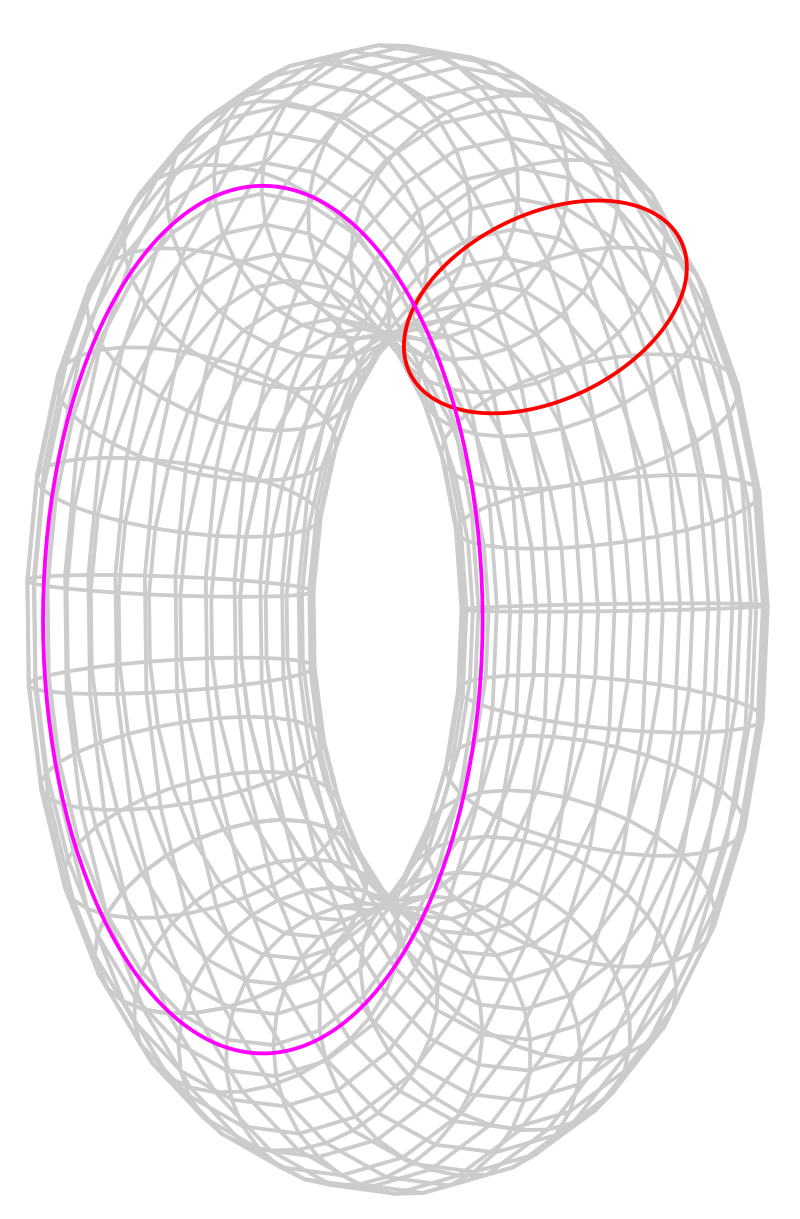
\includegraphics[width=5cm,height=5cm]{torus.png}
https://upload.wikimedia.org/wikipedia/commons/8/81/Torus\_cycles.svg
\end{figure}

In order to acheive this in the sequential version, we pad our 2D grid with additional rows and columns - one additional row on the 
top and one additional row on the bottom. Likewise, we have one additional column on the left and one additional 
column on the right. The height and width variables in life\textunderscore{}seq.c include these padding rows and columns. These 
additional rows and columns contain copies of the values on the edges of the grid. 

The main game of life logic is implemented in a function called evolve.  

\subsection{Parallelization Considerations}
\label{sec:orgee52928}

We want to use MPI Collectives to parallelize the sequential version of the code. 
In order to do this, we have to think about the following things: 

\begin{enumerate}
\item How will we decompose our domain?
\item How can we distribute data between different processes?
\item Do we need to change any of the code from the sequential version?
\end{enumerate}

One of the first ideas you might have for the decomposition might be similar to the last assignment, splitting along the rows and sending one or more rows to each process. This is a good strategy and you should consider using it. Note that this time around, the number of rows is not neatly divisible by the number of processes.\\
However, you are also welcome to try any other strategy you might want. Additionally, you might want to look into 
using MPI's virtual topologies, like a cartesian grid, to help you acheive this. However, this is a more advanced topic and certainly not required. 

To distribute data between different processes, you might want to employ the halo/ghost cell pattern. This can be quite
helpful for iterative stencil codes, such as the Game of Life or a Jacobi solver, where at the boundary of each
domain, we need data from another process. To do this, each process allocates additional space for data that it needs
from neighboring processes - we call these ghost cells. For more details, please refer to this \href{http://fredrikbk.com/publications/ghost\_cell\_pattern.pdf}{excellent introduction}.

To answer the third question, depending on how you parallelize your code, you might need to also modify some functions from Utility.cpp since it does not take into account any domain decompositions that you might perform. To do this, copy the function over to your code, rename it and modify it.


\section{Running your code}
\label{sec:org7d813a7}

\subsection{Normal Operation}
\label{sec:org6bdd59d}
As with the first assignment, please try to run your code with the following signature:

\begin{verbatim}
mpirun -np <num procs> <path to executable>
\end{verbatim}

Both Utility.cpp and VideoOutput.cpp contain some useful methods to help you visualize/analyze what your code is doing.

\subsection{Video Output}
\label{sec:orga32caab}

This assignment also comes with an improved version of the Video/Picture Output. To activate it, you can use the \texttt{-g} option to write video and image output. The video output requires FFMPEG to be available on your path. In this improved version, the video should now be viewable in more media players. As an alternative, it is now also possible to export single frames to PNG. This should no longer require additional dependencies.

\begin{verbatim}
./sequential_implementation -g
\end{verbatim}

While it is not required for this assignment, you can also do this for your parallelized code. To do this, call the relevant video output functions only on rank 0.

Make sure to conduct any timing experiments with visualization disabled.

\section{Speedup requirements}
\label{sec:org2b70086}

Your parallel code, without any visualization output, should be able to acheive a \emph{minimum} speedup of \textbf{13} with \textbf{16 processes}.  

\section{Assignment Deadline}
\label{sec:org8396d51}

The deadline for this assignment is on the \textbf{20th of July at 23:59.} 
\end{document}
